% Options for packages loaded elsewhere
\PassOptionsToPackage{unicode}{hyperref}
\PassOptionsToPackage{hyphens}{url}
\PassOptionsToPackage{dvipsnames,svgnames,x11names}{xcolor}
%
\documentclass[
  letterpaper,
  DIV=11,
  numbers=noendperiod]{scrreprt}

\usepackage{amsmath,amssymb}
\usepackage{iftex}
\ifPDFTeX
  \usepackage[T1]{fontenc}
  \usepackage[utf8]{inputenc}
  \usepackage{textcomp} % provide euro and other symbols
\else % if luatex or xetex
  \usepackage{unicode-math}
  \defaultfontfeatures{Scale=MatchLowercase}
  \defaultfontfeatures[\rmfamily]{Ligatures=TeX,Scale=1}
\fi
\usepackage{lmodern}
\ifPDFTeX\else  
    % xetex/luatex font selection
\fi
% Use upquote if available, for straight quotes in verbatim environments
\IfFileExists{upquote.sty}{\usepackage{upquote}}{}
\IfFileExists{microtype.sty}{% use microtype if available
  \usepackage[]{microtype}
  \UseMicrotypeSet[protrusion]{basicmath} % disable protrusion for tt fonts
}{}
\makeatletter
\@ifundefined{KOMAClassName}{% if non-KOMA class
  \IfFileExists{parskip.sty}{%
    \usepackage{parskip}
  }{% else
    \setlength{\parindent}{0pt}
    \setlength{\parskip}{6pt plus 2pt minus 1pt}}
}{% if KOMA class
  \KOMAoptions{parskip=half}}
\makeatother
\usepackage{xcolor}
\setlength{\emergencystretch}{3em} % prevent overfull lines
\setcounter{secnumdepth}{5}
% Make \paragraph and \subparagraph free-standing
\ifx\paragraph\undefined\else
  \let\oldparagraph\paragraph
  \renewcommand{\paragraph}[1]{\oldparagraph{#1}\mbox{}}
\fi
\ifx\subparagraph\undefined\else
  \let\oldsubparagraph\subparagraph
  \renewcommand{\subparagraph}[1]{\oldsubparagraph{#1}\mbox{}}
\fi

\usepackage{color}
\usepackage{fancyvrb}
\newcommand{\VerbBar}{|}
\newcommand{\VERB}{\Verb[commandchars=\\\{\}]}
\DefineVerbatimEnvironment{Highlighting}{Verbatim}{commandchars=\\\{\}}
% Add ',fontsize=\small' for more characters per line
\usepackage{framed}
\definecolor{shadecolor}{RGB}{241,243,245}
\newenvironment{Shaded}{\begin{snugshade}}{\end{snugshade}}
\newcommand{\AlertTok}[1]{\textcolor[rgb]{0.68,0.00,0.00}{#1}}
\newcommand{\AnnotationTok}[1]{\textcolor[rgb]{0.37,0.37,0.37}{#1}}
\newcommand{\AttributeTok}[1]{\textcolor[rgb]{0.40,0.45,0.13}{#1}}
\newcommand{\BaseNTok}[1]{\textcolor[rgb]{0.68,0.00,0.00}{#1}}
\newcommand{\BuiltInTok}[1]{\textcolor[rgb]{0.00,0.23,0.31}{#1}}
\newcommand{\CharTok}[1]{\textcolor[rgb]{0.13,0.47,0.30}{#1}}
\newcommand{\CommentTok}[1]{\textcolor[rgb]{0.37,0.37,0.37}{#1}}
\newcommand{\CommentVarTok}[1]{\textcolor[rgb]{0.37,0.37,0.37}{\textit{#1}}}
\newcommand{\ConstantTok}[1]{\textcolor[rgb]{0.56,0.35,0.01}{#1}}
\newcommand{\ControlFlowTok}[1]{\textcolor[rgb]{0.00,0.23,0.31}{#1}}
\newcommand{\DataTypeTok}[1]{\textcolor[rgb]{0.68,0.00,0.00}{#1}}
\newcommand{\DecValTok}[1]{\textcolor[rgb]{0.68,0.00,0.00}{#1}}
\newcommand{\DocumentationTok}[1]{\textcolor[rgb]{0.37,0.37,0.37}{\textit{#1}}}
\newcommand{\ErrorTok}[1]{\textcolor[rgb]{0.68,0.00,0.00}{#1}}
\newcommand{\ExtensionTok}[1]{\textcolor[rgb]{0.00,0.23,0.31}{#1}}
\newcommand{\FloatTok}[1]{\textcolor[rgb]{0.68,0.00,0.00}{#1}}
\newcommand{\FunctionTok}[1]{\textcolor[rgb]{0.28,0.35,0.67}{#1}}
\newcommand{\ImportTok}[1]{\textcolor[rgb]{0.00,0.46,0.62}{#1}}
\newcommand{\InformationTok}[1]{\textcolor[rgb]{0.37,0.37,0.37}{#1}}
\newcommand{\KeywordTok}[1]{\textcolor[rgb]{0.00,0.23,0.31}{#1}}
\newcommand{\NormalTok}[1]{\textcolor[rgb]{0.00,0.23,0.31}{#1}}
\newcommand{\OperatorTok}[1]{\textcolor[rgb]{0.37,0.37,0.37}{#1}}
\newcommand{\OtherTok}[1]{\textcolor[rgb]{0.00,0.23,0.31}{#1}}
\newcommand{\PreprocessorTok}[1]{\textcolor[rgb]{0.68,0.00,0.00}{#1}}
\newcommand{\RegionMarkerTok}[1]{\textcolor[rgb]{0.00,0.23,0.31}{#1}}
\newcommand{\SpecialCharTok}[1]{\textcolor[rgb]{0.37,0.37,0.37}{#1}}
\newcommand{\SpecialStringTok}[1]{\textcolor[rgb]{0.13,0.47,0.30}{#1}}
\newcommand{\StringTok}[1]{\textcolor[rgb]{0.13,0.47,0.30}{#1}}
\newcommand{\VariableTok}[1]{\textcolor[rgb]{0.07,0.07,0.07}{#1}}
\newcommand{\VerbatimStringTok}[1]{\textcolor[rgb]{0.13,0.47,0.30}{#1}}
\newcommand{\WarningTok}[1]{\textcolor[rgb]{0.37,0.37,0.37}{\textit{#1}}}

\providecommand{\tightlist}{%
  \setlength{\itemsep}{0pt}\setlength{\parskip}{0pt}}\usepackage{longtable,booktabs,array}
\usepackage{calc} % for calculating minipage widths
% Correct order of tables after \paragraph or \subparagraph
\usepackage{etoolbox}
\makeatletter
\patchcmd\longtable{\par}{\if@noskipsec\mbox{}\fi\par}{}{}
\makeatother
% Allow footnotes in longtable head/foot
\IfFileExists{footnotehyper.sty}{\usepackage{footnotehyper}}{\usepackage{footnote}}
\makesavenoteenv{longtable}
\usepackage{graphicx}
\makeatletter
\def\maxwidth{\ifdim\Gin@nat@width>\linewidth\linewidth\else\Gin@nat@width\fi}
\def\maxheight{\ifdim\Gin@nat@height>\textheight\textheight\else\Gin@nat@height\fi}
\makeatother
% Scale images if necessary, so that they will not overflow the page
% margins by default, and it is still possible to overwrite the defaults
% using explicit options in \includegraphics[width, height, ...]{}
\setkeys{Gin}{width=\maxwidth,height=\maxheight,keepaspectratio}
% Set default figure placement to htbp
\makeatletter
\def\fps@figure{htbp}
\makeatother
\newlength{\cslhangindent}
\setlength{\cslhangindent}{1.5em}
\newlength{\csllabelwidth}
\setlength{\csllabelwidth}{3em}
\newlength{\cslentryspacingunit} % times entry-spacing
\setlength{\cslentryspacingunit}{\parskip}
\newenvironment{CSLReferences}[2] % #1 hanging-ident, #2 entry spacing
 {% don't indent paragraphs
  \setlength{\parindent}{0pt}
  % turn on hanging indent if param 1 is 1
  \ifodd #1
  \let\oldpar\par
  \def\par{\hangindent=\cslhangindent\oldpar}
  \fi
  % set entry spacing
  \setlength{\parskip}{#2\cslentryspacingunit}
 }%
 {}
\usepackage{calc}
\newcommand{\CSLBlock}[1]{#1\hfill\break}
\newcommand{\CSLLeftMargin}[1]{\parbox[t]{\csllabelwidth}{#1}}
\newcommand{\CSLRightInline}[1]{\parbox[t]{\linewidth - \csllabelwidth}{#1}\break}
\newcommand{\CSLIndent}[1]{\hspace{\cslhangindent}#1}

\KOMAoption{captions}{tableheading}
\makeatletter
\makeatother
\makeatletter
\@ifpackageloaded{bookmark}{}{\usepackage{bookmark}}
\makeatother
\makeatletter
\@ifpackageloaded{caption}{}{\usepackage{caption}}
\AtBeginDocument{%
\ifdefined\contentsname
  \renewcommand*\contentsname{Table of contents}
\else
  \newcommand\contentsname{Table of contents}
\fi
\ifdefined\listfigurename
  \renewcommand*\listfigurename{List of Figures}
\else
  \newcommand\listfigurename{List of Figures}
\fi
\ifdefined\listtablename
  \renewcommand*\listtablename{List of Tables}
\else
  \newcommand\listtablename{List of Tables}
\fi
\ifdefined\figurename
  \renewcommand*\figurename{Figura}
\else
  \newcommand\figurename{Figura}
\fi
\ifdefined\tablename
  \renewcommand*\tablename{Tabla}
\else
  \newcommand\tablename{Tabla}
\fi
}
\@ifpackageloaded{float}{}{\usepackage{float}}
\floatstyle{ruled}
\@ifundefined{c@chapter}{\newfloat{codelisting}{h}{lop}}{\newfloat{codelisting}{h}{lop}[chapter]}
\floatname{codelisting}{Listing}
\newcommand*\listoflistings{\listof{codelisting}{List of Listings}}
\makeatother
\makeatletter
\@ifpackageloaded{caption}{}{\usepackage{caption}}
\@ifpackageloaded{subcaption}{}{\usepackage{subcaption}}
\makeatother
\makeatletter
\@ifpackageloaded{tcolorbox}{}{\usepackage[skins,breakable]{tcolorbox}}
\makeatother
\makeatletter
\@ifundefined{shadecolor}{\definecolor{shadecolor}{rgb}{.97, .97, .97}}
\makeatother
\makeatletter
\makeatother
\makeatletter
\makeatother
\ifLuaTeX
  \usepackage{selnolig}  % disable illegal ligatures
\fi
\IfFileExists{bookmark.sty}{\usepackage{bookmark}}{\usepackage{hyperref}}
\IfFileExists{xurl.sty}{\usepackage{xurl}}{} % add URL line breaks if available
\urlstyle{same} % disable monospaced font for URLs
\hypersetup{
  pdftitle={Bestiario de Teoría de Números},
  pdfauthor={Enrique Pérez Herrero},
  colorlinks=true,
  linkcolor={blue},
  filecolor={Maroon},
  citecolor={Blue},
  urlcolor={Blue},
  pdfcreator={LaTeX via pandoc}}

\title{Bestiario de Teoría de Números}
\author{Enrique Pérez Herrero}
\date{2023-10-15}

\begin{document}
\maketitle
\ifdefined\Shaded\renewenvironment{Shaded}{\begin{tcolorbox}[breakable, boxrule=0pt, interior hidden, borderline west={3pt}{0pt}{shadecolor}, enhanced, sharp corners, frame hidden]}{\end{tcolorbox}}\fi

\renewcommand*\contentsname{Table of contents}
{
\hypersetup{linkcolor=}
\setcounter{tocdepth}{2}
\tableofcontents
}
\bookmarksetup{startatroot}

\hypertarget{preuxe1mbulo}{%
\chapter*{Preámbulo}\label{preuxe1mbulo}}
\addcontentsline{toc}{chapter}{Preámbulo}

\markboth{Preámbulo}{Preámbulo}

\bookmarksetup{startatroot}

\hypertarget{intro}{%
\chapter{INTRODUCCION}\label{intro}}

\bookmarksetup{startatroot}

\hypertarget{series-convergentes}{%
\chapter{SERIES CONVERGENTES}\label{series-convergentes}}

En esta parte del libro
\url{https://archive.siam.org/journals/problems/downloadfiles/07-003s.pdf}

\hypertarget{series-que-incluyen-las-funciones-de-parte-entera.}{%
\section{Series que incluyen las funciones de parte
entera.}\label{series-que-incluyen-las-funciones-de-parte-entera.}}

\begin{longtable}[]{@{}
  >{\raggedleft\arraybackslash}p{(\columnwidth - 8\tabcolsep) * \real{0.0171}}
  >{\raggedright\arraybackslash}p{(\columnwidth - 8\tabcolsep) * \real{0.0571}}
  >{\raggedright\arraybackslash}p{(\columnwidth - 8\tabcolsep) * \real{0.2514}}
  >{\raggedright\arraybackslash}p{(\columnwidth - 8\tabcolsep) * \real{0.4800}}
  >{\raggedright\arraybackslash}p{(\columnwidth - 8\tabcolsep) * \real{0.1943}}@{}}
\caption{Fracciones enteras de \(n^2\)}\tabularnewline
\toprule\noalign{}
\begin{minipage}[b]{\linewidth}\raggedleft
k
\end{minipage} & \begin{minipage}[b]{\linewidth}\raggedright
Secuencia
\end{minipage} & \begin{minipage}[b]{\linewidth}\raggedright
Fórmula
\end{minipage} & \begin{minipage}[b]{\linewidth}\raggedright
Descripción
\end{minipage} & \begin{minipage}[b]{\linewidth}\raggedright
Términos
\end{minipage} \\
\midrule\noalign{}
\endfirsthead
\toprule\noalign{}
\begin{minipage}[b]{\linewidth}\raggedleft
k
\end{minipage} & \begin{minipage}[b]{\linewidth}\raggedright
Secuencia
\end{minipage} & \begin{minipage}[b]{\linewidth}\raggedright
Fórmula
\end{minipage} & \begin{minipage}[b]{\linewidth}\raggedright
Descripción
\end{minipage} & \begin{minipage}[b]{\linewidth}\raggedright
Términos
\end{minipage} \\
\midrule\noalign{}
\endhead
\bottomrule\noalign{}
\endlastfoot
1 & \href{https://oeis.org/A000290/}{A000290} &
\(\left\lfloor\frac{n^2}{1}\right\rfloor\) & The squares: a(n) = n\^{}2.
& \{1,4,9,16,25,36,49,64,81,100,\ldots\} \\
2 & \href{https://oeis.org/A007590/}{A007590} &
\(\left\lfloor\frac{n^2}{2}\right\rfloor\) & a(n) = floor(n\^{}2/2). &
\{0,2,4,8,12,18,24,32,40,50,\ldots\} \\
3 & \href{https://oeis.org/A000212/}{A000212} &
\(\left\lfloor\frac{n^2}{3}\right\rfloor\) & a(n) = floor(n\^{}2/3). &
\{0,1,3,5,8,12,16,21,27,33,\ldots\} \\
4 & \href{https://oeis.org/A002620/}{A002620} &
\(\left\lfloor\frac{n^2}{4}\right\rfloor\) & Quarter-squares: a(n) =
floor(n/2)*ceiling(n/2). Equivalently, a(n) = floor(n\^{}2/4). &
\{0,1,2,4,6,9,12,16,20,25,\ldots\} \\
5 & \href{https://oeis.org/A118015/}{A118015} &
\(\left\lfloor\frac{n^2}{5}\right\rfloor\) & a(n) = floor(n\^{}2/5). &
\{0,0,1,3,5,7,9,12,16,20,\ldots\} \\
6 & \href{https://oeis.org/A056827/}{A056827} &
\(\left\lfloor\frac{n^2}{6}\right\rfloor\) & a(n) = floor(n\^{}2/6). &
\{0,0,1,2,4,6,8,10,13,16,\ldots\} \\
7 & \href{https://oeis.org/A056834/}{A056834} &
\(\left\lfloor\frac{n^2}{7}\right\rfloor\) & a(n) = floor(n\^{}2/7). &
\{0,0,1,2,3,5,7,9,11,14,\ldots\} \\
8 & \href{https://oeis.org/A130519/}{A130519} &
\(\left\lfloor\frac{n^2}{8}\right\rfloor\) & a(n) = Sum\_\{k=0..n\}
floor(k/4). (Partial sums of A002265.) &
\{0,0,1,2,3,4,6,8,10,12,\ldots\} \\
9 & \href{https://oeis.org/A056838/}{A056838} &
\(\left\lfloor\frac{n^2}{9}\right\rfloor\) & a(n) = floor(n\^{}2/9). &
\{0,0,1,1,2,4,5,7,9,11,\ldots\} \\
10 & \href{https://oeis.org/A056865/}{A056865} &
\(\left\lfloor\frac{n^2}{10}\right\rfloor\) & a(n) = floor(n\^{}2/10). &
\{0,0,0,1,2,3,4,6,8,10,\ldots\} \\
\end{longtable}

\hypertarget{funciuxf3n-techo-de-n2-medios-a000982}{%
\subsection{\texorpdfstring{Función techo de \(n^2\) medios,
\href{https://oeis.org/A000982}{A000982}}{Función techo de n\^{}2 medios, A000982}}\label{funciuxf3n-techo-de-n2-medios-a000982}}

\begin{equation}\protect\hypertarget{eq-A000982}{}{
A000982 = \left\{ 0, 1, 2, 5, 8, 13, 18, 25, 32, 41, 50, 61, 72, 85, 98, 113, 128 , \dots \right\}
}\label{eq-A000982}\end{equation}

\begin{equation}\protect\hypertarget{eq-A000982-b}{}{
A000982(n) = \left\lceil  \frac{n^2}{2} \right\rceil
}\label{eq-A000982-b}\end{equation}

\begin{itemize}
\tightlist
\item
  \textbf{Problema} - Sumar la serie:
\end{itemize}

\begin{equation}\protect\hypertarget{eq-A000982-a}{}{
\sum_{n=1}^{\infty}{\frac{1}{\left\lceil  \frac{n^2}{2} \right\rceil}}
}\label{eq-A000982-a}\end{equation}

\begin{itemize}
\tightlist
\item
  \textbf{Solución}:
\end{itemize}

Para sumar la serie infinita, separamos la secuencia en otras dos, una
que contiene los términos pares y la otra los impares.

\begin{equation}\protect\hypertarget{eq-A001105}{}{
A001105(n) = 2n^2
}\label{eq-A001105}\end{equation}

\begin{equation}\protect\hypertarget{eq-A001844}{}{
A001844(n) = 2n(n+1) + 1
}\label{eq-A001844}\end{equation}

Referencia a la ecuación Ecuación~\ref{eq-A001844}

\begin{multline}
\sum_{n=1}^{\infty}{\frac{1}{\left\lceil \frac{n^2}{2} \right\rceil}} =  \sum_{m=1}^{\infty}{\frac{1}{2m^2}}  + \sum_{m=0}^{\infty}{\frac{1}{2m(m+1) + 1}} 
  (\#eq:A000982-c)
\end{multline}

\begin{multline}
\sum_{n=1}^{\infty}{\frac{1}{\left\lceil \frac{n^2}{2} \right\rceil}} =  \frac{\zeta(2)}{2} + \frac{\pi}{2} \cdot \tanh\left(\frac{\pi}{2}\right)
  (\#eq:A000982-d)
\end{multline}

\hypertarget{funciuxf3n-suelo-de-n2-tercios-a000212}{%
\subsection{\texorpdfstring{Función suelo de \(n^2\) tercios,
\href{https://oeis.org/A000212}{A000212}}{Función suelo de n\^{}2 tercios, A000212}}\label{funciuxf3n-suelo-de-n2-tercios-a000212}}

\[A000212 = \left\{ 0, 0, 1, 3, 5, 8, 12, 16, 21, 27, 33, 40, 48, 56, 65, 75 , \dots \right\}\]

\begin{itemize}
\tightlist
\item
  \textbf{Problema}: Sumar la serie:
\end{itemize}

\begin{equation}\protect\hypertarget{eq-A000212-a}{}{
\begin{multline}
\sum_{n=2}^{\infty}{\frac{1}{\left\lfloor \frac{n^2}{3} \right\rfloor}}
\end{multline}
}\label{eq-A000212-a}\end{equation}

\begin{itemize}
\tightlist
\item
  \textbf{Solución}:
\end{itemize}

\begin{equation}\protect\hypertarget{eq-A000212-b}{}{
\begin{multline}
A000212(n) = \left\lfloor \frac{n^2}{3} \right\rfloor
\end{multline}
}\label{eq-A000212-b}\end{equation}

Separamos la secuencia problema, en tres secuencias, para sumarlas por
separado

\begin{itemize}
\tightlist
\item
  Números octagonales: \href{https://oeis.org/A000567}{A000567}:
\end{itemize}

\begin{equation}\protect\hypertarget{eq-A000567-a}{}{
\begin{multline}
\!\begin{aligned}
\left\lfloor \frac{(3m+2)^{2}}{3} \right\rfloor \\
& =  A000567(m) \\
& = \{1, 8, 21, 40, 65, 96, 133, 176, 225, 280, 341, 408, 481, 560,...\} \\
& = m(3m-2)
\end{aligned}
\end{multline}
}\label{eq-A000567-a}\end{equation}

\begin{equation}\protect\hypertarget{eq-A000567-b}{}{
\begin{multline}
\sum_{m=1}^{\infty}{\frac{1}{m(3m-2)}} = \frac{1}{12} (\pi\sqrt{3} + 9\log{3}) 
\end{multline}
}\label{eq-A000567-b}\end{equation}

\begin{itemize}
\tightlist
\item
  Números rómbicos: \href{https://oeis.org/A045944}{A045944}:
\end{itemize}

\begin{equation}\protect\hypertarget{eq-A045944-a}{}{
\begin{multline}
\!\begin{aligned}
\left\lfloor \frac{(3m+1)^{2}}{3} \right\rfloor \\
& =  A045944(m) \\
& = \{5, 16, 33, 56, 85, 120, 161, 208, 261, 320, 385, 456, 533,...\} \\
& = m(3m+2)
\end{aligned}
\end{multline}
}\label{eq-A045944-a}\end{equation}

\begin{multline}
\sum_{m=1}^{\infty}{\frac{1}{m(3m+2)}} = 
\frac{1}{12} (9 + \pi\sqrt{3} - 9\log{3}) 
  (\#eq:A045944-b)
\end{multline}

\begin{itemize}
\tightlist
\item
  Secuencia \(3n^2\) \href{https://oeis.org/A033428}{A033428}:
\end{itemize}

\begin{multline}
\!\begin{aligned}
\left\lfloor \frac{(3m)^{2}}{3} \right\rfloor \\
& =  A033428(m) \\
& = \{3, 12, 27, 48, 75, 108, 147, 192, 243, 300, 363, 432, 507,...\} \\
& = 3m^2
\end{aligned}
  (\#eq:A033428-a)
\end{multline}

\begin{multline}
\sum_{m=1}^{\infty}{\frac{1}{3m^2}} = \frac{\zeta(2)}{3} = \frac{\pi^2}{18}
  (\#eq:A033428-b)
\end{multline}

\begin{multline}
\sum_{n=2}^{\infty}{\frac{1}{\left\lfloor \frac{n^2}{3} \right\rfloor}} = 
\frac{1}{36} \left(6 \pi  \sqrt{3}+2 \pi ^2+27\right)
(\#eq:A000212-c)
\end{multline}

\begin{itemize}
\tightlist
\item
  Código para \emph{Wolfram Mathematica}
\end{itemize}

\begin{Shaded}
\begin{Highlighting}[]
\NormalTok{    S1 = Sum[1/(m*(3 m {-} 2)), \{m, 1, Infinity\}];}
\NormalTok{    S2 = Sum[1/(m*(3 m + 2)), \{m, 1, Infinity\}];}
\NormalTok{    S3 = Sum[1/(3*m\^{}2), \{m, 1, Infinity\}];}
\NormalTok{    S = Simplify[S1 + S2 + S3];}
\NormalTok{    S}
\end{Highlighting}
\end{Shaded}

\hypertarget{cuartos-cuadrados-index-1-secuencia-a002620}{%
\subsection[Cuartos cuadrados , secuencia
\href{https://oeis.org/A002620}{A002620}]{\texorpdfstring{Cuartos
cuadrados \footnote{La función
  \(f(t) = \left\lfloor t \right\rfloor \left\lceil  t \right\rceil\),
  es simétrica respecto a origen \(f(-t)=f(t)\)}, secuencia
\href{https://oeis.org/A002620}{A002620}}{Cuartos cuadrados , secuencia A002620}}\label{cuartos-cuadrados-index-1-secuencia-a002620}}

\[A002620 = \{0, 0, 1, 2, 4, 6, 9, 12, 16, 20, 25, 30, 36, 42, 49, 56,...\}\]
Se puede observar como los términos pares de la secuencia se
corresponden a los cuadrados perfectos
(\href{https://oeis.org/A000290}{A000290}), mientras que los términos
impares son los números oblongos
(\href{https://oeis.org/A002378}{A002378}).

\begin{multline}
A002620(n) = \left\lfloor \frac{n^2}{4} \right\rfloor = 
\left\lfloor \frac{n^2}{2} \right\rfloor \cdot \left\lceil \frac{n^2}{2} \right\rceil
  (\#eq:A002620-a)
\end{multline}

\begin{multline}
\!\begin{aligned}
\sum_{n=2}^{\infty}{\frac{1}{A002620(n)}} & = \sum_{n=2}^{\infty}{\frac{1}{ \left\lfloor\frac{n^2}{4}\right\rfloor}} \\
& = \sum_{m=1}^{\infty}{\frac{1}{m^2}} + \sum_{m=1}^{\infty}{\frac{1}{m(m+1)}} \\
& = \zeta(2) + 1 \\
& = \frac{\pi^2}{6} + 1
\end{aligned}
(\#eq:A002620-b)
\end{multline}

\hypertarget{generalizaciuxf3n}{%
\subsection{Generalización}\label{generalizaciuxf3n}}

\begin{multline}
\begin{split}
S(k) & =
\sum_{n=\lceil \sqrt{k} \rceil}^{\infty}{\frac{1}{\left\lfloor\frac{n^2}{k}\right\rfloor}} \\
& = \sum_{s=0}^{k-1}{\sum_{m=[{s}^{2} \lt k]}^{\infty}\frac{1}{\left\lfloor\frac{{(k m + s)}^{2}}{k}\right\rfloor}} \\

& = \frac{\zeta(2)}{k} + \sum_{s=1}^{k-1}{\sum_{m=[s^2 \lt k]}^{\infty}\frac{1}{\left\lfloor\frac{{(k m + s)}^{2}}{k}\right\rfloor}}
\end{split}
(\#eq:gener)
\end{multline}

\hypertarget{series-relacionadas-con-nuxfameros-figurativos}{%
\section{Series relacionadas con números
figurativos}\label{series-relacionadas-con-nuxfameros-figurativos}}

Los \textbf{números figurativos} son números que pueden representarse
como una disposición geométrica regular de puntos separados de forma
idéntica. La disposición puede ser plana o tridimensional. Por ejemplo,
sí la disposición de los puntos forma un \textbf{polígono regular}
hablamos de \textbf{números poligonales}. También podemos estudiar
disposiciones en forma de \textbf{polihédrica}, como puede ser
piramidal, tetrehédrica, etc.

Se listan, a continuación, varios ejemplos de sumas convergentes,
tomando la suma infinita de los inversos de varios ejemplos de
\textbf{números figurativos}.

\hypertarget{nuxfameros-pentagonales-secuencia-a000326}{%
\subsection{\texorpdfstring{Números Pentagonales, secuencia
\href{https://oeis.org/A000326}{A000326}}{Números Pentagonales, secuencia A000326}}\label{nuxfameros-pentagonales-secuencia-a000326}}

\begin{multline}
A000326(n) = \frac{n(3n-1)}{2}
  (\#eq:A000326-a)
\end{multline}

\begin{multline}
\sum_{n=1}^{\infty}{\frac{1}{A000326(n)}} = 
\sum_{n=1}^{\infty}{\frac{2}{n(3n-1)}} =
\frac{1}{3} \left(9 \log (3)-\sqrt{3} \pi \right)
  (\#eq:A000326-b)
\end{multline}

Los dígitos de la expansión decimal, de la constante obtenida, de la
suma de los recíprocos de los \textbf{números pentagonales} corresponde
a la secuencia: \href{https://oeis.org/A244641}{A244641}

\begin{itemize}
\tightlist
\item
  Código para \emph{Wolfram Mathematica}:
\end{itemize}

\begin{Shaded}
\begin{Highlighting}[]
\NormalTok{    A000326[n\_] := n(3n{-}1)/2}
\NormalTok{    Sum[1/A000326[n], \{n, 1, Infinity\}]}
\end{Highlighting}
\end{Shaded}

\hypertarget{nuxfameros-hexagonales-secuencia-a000384}{%
\subsection{\texorpdfstring{Números Hexagonales, secuencia
\href{https://oeis.org/A000384}{A000384}}{Números Hexagonales, secuencia A000384}}\label{nuxfameros-hexagonales-secuencia-a000384}}

\begin{multline}
A000384(n) = n(2n-1)
  (\#eq:A000384-a)
\end{multline}

\begin{multline}
\sum_{n=1}^{\infty}{\frac{1}{A000384(n)}} = 
\sum_{n=1}^{\infty}{\frac{1}{n(2n-1)}} = 
2\log(2)
  (\#eq:A000384-b)
\end{multline}

La expansión decimal de \(2\log(2)\) corresponde a la secuencia
\href{https://oeis.org/A016627}{A016627}

\begin{itemize}
\tightlist
\item
  Código para \emph{Wolfram Mathematica}:
\end{itemize}

\begin{Shaded}
\begin{Highlighting}[]
\NormalTok{    A000384[n\_] := n(2n{-}1)}
\NormalTok{    Sum[1/A000384[n], \{n, 1, Infinity\}]}
\end{Highlighting}
\end{Shaded}

\hypertarget{nuxfameros-piramidales-de-base-cuadrada-secuencia-a000330}{%
\subsection{\texorpdfstring{Números Piramidales de Base Cuadrada,
secuencia
\href{https://oeis.org/A000330}{A000330}}{Números Piramidales de Base Cuadrada, secuencia A000330}}\label{nuxfameros-piramidales-de-base-cuadrada-secuencia-a000330}}

La secuencia \href{https://oeis.org/A000330}{A000330} viene definida por
la \href{https://mathworld.wolfram.com/FaulhabersFormula.html}{fórmula
de Faulhaber} para la suma de los \(n\) primeros \textbf{cuadrados
perfectos}.

\begin{multline}
A000330(n)=\sum_{k=1}^{n}{k^2}=\frac{n(n+1)(2n+1)}{6}
  (\#eq:A000330-a)
\end{multline}

Para calcular la \textbf{suma infinita} de los inversos de los
\textbf{números piramidales de base cuadrada}:

\begin{multline}
   \sum_{k=1}^{\infty}{\frac{6}{k(k+1)(2k+1)}}
  (\#eq:A000330-b)
\end{multline}

Nos basamos en la \textbf{suma finita} de los \(n\) primeros
\textbf{números piramidales de base cuadrada} que es:

\begin{multline}
   S(n)=\sum_{k=1}^{n}{\frac{6}{k(k+1)(2k+1)}}
  (\#eq:A000330-c)
\end{multline}

Separando la fracción principal en otras con denominador de grado uno en
\(k\):

\begin{multline}
\frac{S(n)}{6}=
\sum_{k=1}^{n}{\frac{1}{k(k+1)(2k+1)}} =
\sum_{k=1}^{n}{\frac{A}{k}+\frac{B}{k+1}+\frac{C}{2k+1}}
 (\#eq:A000330-d)
\end{multline}

Y resolviendo el sistema de ecuaciones, se obtiene:

\begin{multline}
A=1 ;\; B=1;\; C=-4;
 (\#eq:A000330-e)
\end{multline}

Sustituyendo en la serie problema, los valores obtenidos
@ref(eq:A000330-e), la expresión de los \textbf{números armónicos}
@ref(eq:armonicos1) y teniendo en cuenta la suma de la
serie@ref(eq:armonicos2):

\begin{multline}
\displaystyle \frac{S(n)}{6}= \sum_{k=1}^{n} {\frac{1}{k}}+\sum_{k=1}^{n}{\frac{1}{k+1}}-4\sum_{k=1}^{n}{\frac{1}{2k+1}}
= 2H_{n}-\frac{n}{n+1}-4\sum_{k=1}^{n}{\frac{1}{2k+1}}
 (\#eq:A000330-f)
\end{multline}

Considerando las expresiones @ref(eq:armonicos1), @ref(eq:digamma1) y
que cumple la función digamma \(\psi_{0}\):

Taking into account the expressions: (i),(iv) and (vi), for the digamma
function:

\begin{multline}
\frac{S(n)}{6} = 2\gamma + 2\psi_{0}(n+1) - \frac{n}{n+1}
- 4\sum_{k=1}^{n}{\frac{1}{2k+1}}
 (\#eq:A000330-g)
\end{multline}

\begin{multline}
S(n) = 6(2\gamma+2\psi_{0}(n+1) -\frac{n}{n+1}-2(\psi_{0}(n+\frac{3}{2})+\gamma+2\log(2)-2))
 (\#eq:A000330-h)
\end{multline}

\begin{multline}
S(n)=6(2\psi_{0}(n+1)-2\psi_{0}(n+\frac{3}{2})-\frac{n}{n+1} -4\log(2)+4)
 (\#eq:A000330-i)
\end{multline}

Calculando el límite y sustituyendo (vii):

\begin{multline}
S(\infty)= \lim_{x \to{+}\infty}{S(n)}= 6(3-4\log(2))
= 18-24\log(2)\approx 1.3644676665...
 (\#eq:A000330-j)
\end{multline}

El resultado de la suma viene recogido en la constante
\href{https://oeis.org/A159354}{A159354}

\begin{multline}
   \sum_{n=1}^{\infty}{\frac{1}{A000330(n)}} = \sum_{n=1}^{\infty}{\frac{6}{n(n+1)(2n+1)}} =
   18-24\log(2) =
   A159354
  (\#eq:A000330-k)
\end{multline}

(véase {[}4{]})

\hypertarget{identidades-usadas-en-la-demostraciuxf3n}{%
\subsubsection{Identidades usadas en la
demostración:}\label{identidades-usadas-en-la-demostraciuxf3n}}

\begin{enumerate}
\def\labelenumi{(\roman{enumi})}
\tightlist
\item
  \emph{Números Armónicos} \(H_{n}\) y
  \href{https://mathworld.wolfram.com/DigammaFunction.html}{función
  digamma} \(\psi_{0}\) para valores enteros:
\end{enumerate}

\begin{multline}
H_{n}=\sum_{k=1}^n {\frac{1}{k}}=\gamma+\psi_{0}(n+1)
(\#eq:armonicos1)
\end{multline}

\begin{enumerate}
\def\labelenumi{(\roman{enumi})}
\setcounter{enumi}{1}
\tightlist
\item
  Incluyendo los \emph{Números Armónicos} en la serie:
\end{enumerate}

\begin{multline}
\sum_{k=1}^{n}{\frac{1}{k+1}}
= \sum_{k=1}^{n}{\frac{1}{k}}-1+\frac{1}{n+1}=H_{n}-\frac{n}{n+1}
(\#eq:armonicos2)
\end{multline}

\begin{enumerate}
\def\labelenumi{(\roman{enumi})}
\setcounter{enumi}{2}
\tightlist
\item
  Changing one series into another:
\end{enumerate}

\begin{multline}
\sum_{k=1}^{n}{\frac{1}{2k-1}} -\sum_{k=1}^{n}{\frac{1}{2k+1}} =
1-\frac{1}{2n+1}
(\#eq:serie1)
\end{multline}

\begin{enumerate}
\def\labelenumi{(\roman{enumi})}
\setcounter{enumi}{3}
\tightlist
\item
  Función digamma para valores semi enteros:
\end{enumerate}

See (\textbf{Knopp1990TheoryAA?})

\begin{multline}
\psi_{0}(n+\frac{1}{2}) = -\gamma-2\log(2)+2\sum_{k=1}^n{\frac{1}{2k-1}}
(\#eq:digamma1)
\end{multline}

\begin{enumerate}
\def\labelenumi{(\alph{enumi})}
\setcounter{enumi}{21}
\tightlist
\item
  La función \emph{Digamma} cumple la propiedad:
\end{enumerate}

\begin{multline}
\psi_{0}(z+1)= \psi_{0}(z)+\frac{1}{z}
(\#eq:digamma2)
\end{multline}

\begin{enumerate}
\def\labelenumi{(\roman{enumi})}
\setcounter{enumi}{5}
\tightlist
\item
  Otra expresión alternativa para la
  \href{https://mathworld.wolfram.com/DigammaFunction.html}{función
  digamma} para valores semi enteros:
\end{enumerate}

Utilizando las ecuaciones (iii), (iv) y (v):

\begin{multline}
\psi_{0}(n+\frac{3}{2}) = 
\psi_{0}(n+\frac{1}{2}) +\frac{1}{n+\frac{1}{2}} = \\ \psi_{0}(n+\frac{1}{2})+\frac{2}{2n+1}=\\
-\gamma-2\log(2) +2(1-\frac{1}{2n+1}+\sum_{k=1}^n{\frac{1}{2k+1}})= \\
-\gamma-2\log(2) +2 +2\sum_{k=1}^{n}{\frac{1}{2k+1}}
(\#eq:digamma3)
\end{multline}

\begin{enumerate}
\def\labelenumi{(\roman{enumi})}
\setcounter{enumi}{6}
\tightlist
\item
  Límite de la función digamma para valores semi enteros:
\end{enumerate}

\begin{multline}
 L_{1}(\infty)=\lim_{x \to{+}\infty}{L_{1}(n)} =
  \lim_{x \to{+}\infty}{[\psi_{0}(n+1)-\psi_{0}(n+\frac{3}{2})] }
(\#eq:digamma4)
\end{multline}

\begin{multline}
L_{1}(n)=\psi_{0}(n+1)-\psi_{0}(n+\frac{3}{2}) =
  2\log(2) + \sum_{k=1}^{n}{\frac{1}{k}}-2 \sum_{k=1}^{n}{\frac{1}{2k-1}} \\
(\#eq:digamma5)
\end{multline}

\begin{multline}
L_{1}(n)=2\log(2)-\sum_{k=1}^{n}{\frac{1}{k(2k-1)}}
(\#eq:digamma6)
\end{multline}

El límite de la serie @ref(eq:digamma6) anterior se puede obtener las
series infinitas de \emph{Mercator-Mengoli} para el desarrollo de la
constante \(\log(2)\), véase {[}3{]}

\begin{multline}
\log(2)=\sum_{k=1}^{\infty}{\frac{1}{2k(2k-1)}}
(\#eq:mercator1)
\end{multline}

Y calculando el límite:

\begin{multline}
L_{1}(\infty)=0
(\#eq:mercator2)
\end{multline}

\bookmarksetup{startatroot}

\hypertarget{funciones-de-la-ciencia-de-la-computaciuxf3n}{%
\chapter{FUNCIONES DE LA CIENCIA DE LA
COMPUTACIÓN}\label{funciones-de-la-ciencia-de-la-computaciuxf3n}}

\[
% Macros del usuario
\renewcommand{\floor}[1] {\lfloor #1 \rfloor}
\renewcommand{\ceil}[1] {\lceil #1 \rceil}
\renewcommand{\fracpart}[1] {\{ #1 \}}
\]

\hypertarget{funciones-de-redondeo}{%
\section{Funciones de redondeo}\label{funciones-de-redondeo}}

Suelo, Techo y Parte Fraccionaria.

\hypertarget{propiedades}{%
\subsection{Propiedades}\label{propiedades}}

\begin{equation}\protect\hypertarget{eq-prop1}{}{
\begin{align}
x =  \left\lfloor x \right\rfloor + \left\{ x \right\}
\end{align}
}\label{eq-prop1}\end{equation}

\hypertarget{integraciuxf3n}{%
\subsection{Integración}\label{integraciuxf3n}}

Las funciones de redondeo de números enteros aparecen en muchos textos
de matemáticas, pero entre la lista de sus propiedades es casi imposible
encontrar nada sobre su integración.

A partir de su representación gráfica es sencillo, añadiendo o
sustrayendo áreas, obtener expresiones de sus \emph{integrales
definidas}, para límites en el intervalo \([0, x]\). Para simplificar
las fórmulas, se pueden emplear los \emph{Números Triangulares},
secuencia \href{https://oeis.org/A000217}{A000217}

\begin{equation}\protect\hypertarget{eq-triang}{}{
\begin{multline}
T(n)=\frac{n^{2}+n}{2}
\end{multline}
}\label{eq-triang}\end{equation}

\hypertarget{integral-definida-de-la-funciuxf3n-suelo}{%
\subsubsection{Integral definida de la función
suelo}\label{integral-definida-de-la-funciuxf3n-suelo}}

\begin{equation}\protect\hypertarget{eq-integralsuelo1}{}{
\begin{align}
I_{1}(x) = \int_0^{x}{\left\lfloor t \right\rfloor dt} =
\left\lfloor x \right\rfloor \left\{ x \right\} + \frac{\left\lfloor x \right\rfloor^2 - \left\lfloor x \right\rfloor}{2} = 
\left\{ x \right\}\left\lfloor x \right\rfloor + T(\left\lfloor x \right\rfloor - 1)
\end{align}
}\label{eq-integralsuelo1}\end{equation}

\hypertarget{integral-definida-de-la-funciuxf3n-parte-fraccionaria}{%
\subsubsection{Integral definida de la función parte
fraccionaria}\label{integral-definida-de-la-funciuxf3n-parte-fraccionaria}}

\begin{equation}\protect\hypertarget{eq-integralfrac1}{}{
\begin{multline}
I_{2}(x) = 
\int_0^x \left\{{t}\right\} dt =
\frac{x}{2} - \left\{ x \right\} + T(\left\{ x \right\}) =
\frac{x}{2} + T(\left\{ x \right\}-1)
\end{multline}
}\label{eq-integralfrac1}\end{equation}

\begin{equation}\protect\hypertarget{eq-integralfrac2}{}{
\begin{multline}
I_{2}(x) = 
\int_0^x \left\{ t \right\} dt =
\frac{\left\lfloor x \right\rfloor + \left\{ x \right\}^{2}}{2} =
\frac{x + \left\{ x \right\}^{2}-\left\{ x \right\}}{2}
\end{multline} 
}\label{eq-integralfrac2}\end{equation}

Los resultados anteriores se pueden modificar empleando la relación
entre ellas véase Ecuación~\ref{eq-prop1}.

\hypertarget{integral-definida-de-la-funciuxf3n-techo}{%
\subsubsection{Integral definida de la función
techo}\label{integral-definida-de-la-funciuxf3n-techo}}

\begin{equation}\protect\hypertarget{eq-integraltecho1}{}{
\begin{multline}
I_{3}(x) = 
\int_{0}^{x}{\left\lceil  x \right\rceil dt} =
\left\lceil  x \right\rceil (x-\left\lceil  x \right\rceil) + T(\left\lceil  x \right\rceil)
\end{multline}
}\label{eq-integraltecho1}\end{equation}

\hypertarget{integral-definida-de-la-parte-entera-al-cuadrado}{%
\subsubsection{Integral definida de la parte entera al
cuadrado}\label{integral-definida-de-la-parte-entera-al-cuadrado}}

\begin{figure}

{\centering 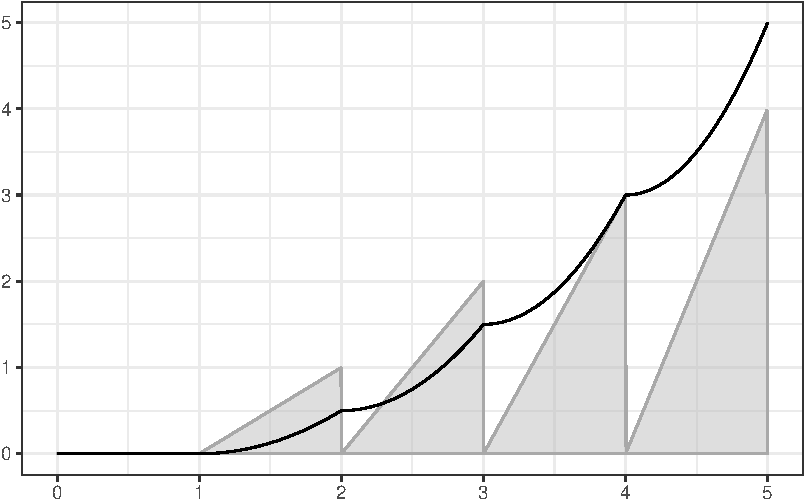
\includegraphics{book/03-Computación/index_files/figure-pdf/unnamed-chunk-2-1.pdf}

}

\caption{Parte entera al cuadrado}

\end{figure}

Para valores positivos de la variable, \(x\geq 0\):

\begin{equation}\protect\hypertarget{eq-integralfrac3}{}{
\begin{multline}
I_{4}(x)= \int_0^x \left\{{t}\right\}^2 dx =
\int_0^{\left\lfloor x \right\rfloor} \left\{{t}\right\}^2 dt +
\int_{{\left\lfloor x \right\rfloor}}^{x} \left\{{t}\right\}^2 dt
\end{multline}
}\label{eq-integralfrac3}\end{equation}

La función \(\left\{ t \right\}^2\) tiene un comportamiento periódico,
por lo que los límites de integración se pueden reducir al primer
periodo. Si \(t \in [0,1]\) entonces \(\left\{ t \right\}^2\) equivale a
\(t^2\).

\begin{equation}\protect\hypertarget{eq-integralfrac4}{}{
\begin{multline}
I_{4}(x)= \int_0^x \left\{{t}\right\}^2 dx =
\int_0^{\left\lfloor x \right\rfloor} \left\{{t}\right\}^2 dt +
\int_{{\left\lfloor x \right\rfloor}}^{x} \left\{{t}\right\}^2 dt
\end{multline}
}\label{eq-integralfrac4}\end{equation}

\begin{equation}\protect\hypertarget{eq-integralfrac5}{}{
\begin{multline}
I_4(x) =
\left\lfloor x \right\rfloor \int_{0}^{1} {\left\{{t}\right\}^2 dt} +
\int_0^{\left\{ x \right\}}{\left\{{t}\right\}^2 dt} = 
\left\lfloor x \right\rfloor \int_{0}^{1}{t^2 dt} + 
\int_0^{\left\{ x \right\}} {t^2 dt}
\end{multline}
}\label{eq-integralfrac5}\end{equation}

\begin{equation}\protect\hypertarget{eq-integralfrac6}{}{
\begin{multline}
I_{4}(x) = \int_0^x \left\{{t}\right\}^2 dt =
\frac{ \left\lfloor x \right\rfloor + \left\{ x \right\}^3}{3} =
\frac{x + \left\{ x \right\}^{3}-\left\{ x \right\}}{3}
\end{multline}
}\label{eq-integralfrac6}\end{equation}

\hypertarget{integral-definida-de-la-parte-entera-a-la-potencia-n}{%
\subsubsection{\texorpdfstring{Integral definida de la parte entera a la
potencia
\(n\)}{Integral definida de la parte entera a la potencia n}}\label{integral-definida-de-la-parte-entera-a-la-potencia-n}}

Empleando el mismo método de cálculo se puede generalizar la fórmula
Ecuación~\ref{eq-integralfrac6} para obtener la integral indefinida de
la parte entera de un número elevado a cualquier potencia entera.

\begin{equation}\protect\hypertarget{eq-integralfrac8}{}{
\begin{multline}
I_{5}(x) = \int_0^x \left\{{t}\right\}^n dt =
\frac{\left\lfloor x \right\rfloor + \left\{ x \right\}^{n+1}}{n+1} =
\frac{x + \left\{ x \right\}^{n+1}-\left\{ x \right\}}{n+1}
\end{multline}
}\label{eq-integralfrac8}\end{equation}

\hypertarget{integral-definida-de-la-funciuxf3n-suelo-al-cuadrado}{%
\subsubsection{Integral definida de la función suelo al
cuadrado}\label{integral-definida-de-la-funciuxf3n-suelo-al-cuadrado}}

\begin{equation}\protect\hypertarget{eq-integralsuelo2a}{}{
\begin{multline}
I_{6}(x) = \int_{0}^{x}{\left\lfloor t \right\rfloor^2 dt} =
\int_{0}^{\left\lfloor x \right\rfloor}{\left\lfloor t \right\rfloor^2 dt} 
+ \int_{{\left\lfloor x \right\rfloor}}^{x}{\left\lfloor t \right\rfloor^2 dt}
\end{multline}
}\label{eq-integralsuelo2a}\end{equation}

\begin{equation}\protect\hypertarget{eq-integralsuelo2b}{}{
\begin{multline}
I_{6}(x) =\sum_{k=1}^{\left\lfloor x \right\rfloor - 1}{k^2} +
\left\{ x \right\}\left\lfloor x \right\rfloor^2 
\end{multline}
}\label{eq-integralsuelo2b}\end{equation}

\begin{equation}\protect\hypertarget{eq-integralsuelo2c}{}{
\begin{multline}
I_{6}(x) = 
P(\left\lfloor x \right\rfloor - 1) + \left\{ x \right\} \left\lfloor x \right\rfloor^2
\end{multline}
}\label{eq-integralsuelo2c}\end{equation}

Dónde \(P(n)\) es el enésimo \emph{Número Piramidal de Base Cuadrada},
secuencia \href{https://oeis.org/A000330}{A000330}

\begin{equation}\protect\hypertarget{eq-piramidal}{}{
\begin{multline}
P(n) =\frac{n(n+1)(2n+1)}{6}
\end{multline}
}\label{eq-piramidal}\end{equation}

\begin{equation}\protect\hypertarget{eq-integralsuelo2dux29}{}{
\begin{multline}
I_{6}(x) = \int_{0}^{x}{\left\lfloor t \right\rfloor^2 dt} = 
\frac{\left\lfloor x \right\rfloor  \left(6 \left\lfloor x \right\rfloor \left\{ x \right\} +
2 \left\lfloor x \right\rfloor^{2} - 3 \left\lfloor x \right\rfloor + 1 \right)}{6}
\end{multline}
}\label{eq-integralsuelo2d)}\end{equation}

\hypertarget{integral-definida-de-la-funciuxf3n-suelo-a-la-potencia-n}{%
\subsubsection{\texorpdfstring{Integral definida de la función suelo a
la potencia
\(n\)}{Integral definida de la función suelo a la potencia n}}\label{integral-definida-de-la-funciuxf3n-suelo-a-la-potencia-n}}

\begin{equation}\protect\hypertarget{eq-integralnsuelo1}{}{
\begin{multline}
I_{7}(x)= \int_{0}^{x}{\left\lfloor t \right\rfloor^{n} dt } =
\sum_{k=1}^{\left\lfloor x \right\rfloor - 1}{k^n} + \left\{ x \right\}\left\lfloor x \right\rfloor^n
\end{multline}
}\label{eq-integralnsuelo1}\end{equation}

\begin{equation}\protect\hypertarget{eq-faulhaber}{}{
\begin{multline}
S(n,m)=\sum_{k=1}^{m}{k^n}
\end{multline}
}\label{eq-faulhaber}\end{equation}

\begin{equation}\protect\hypertarget{eq-integralnsuelo2}{}{
\begin{multline}
I_{7}(x) = \int_0^x \left\lfloor t \right\rfloor^n dt =
S(n, \left\lfloor x \right\rfloor - 1) +
\left\{ x \right\}\left\lfloor x \right\rfloor^n
\end{multline}
}\label{eq-integralnsuelo2}\end{equation}

If \(n=1\) , the formula gives the Triangular Numbers.

And if \(n=2\) , the formula gives the Square Pyramidal Numbers.

\hypertarget{integral-definida-del-producto-de-la-funciuxf3n-suelo-y-la-parte-entera}{%
\subsubsection{Integral definida del producto de la función suelo y la
parte
entera}\label{integral-definida-del-producto-de-la-funciuxf3n-suelo-y-la-parte-entera}}

\begin{figure}

{\centering 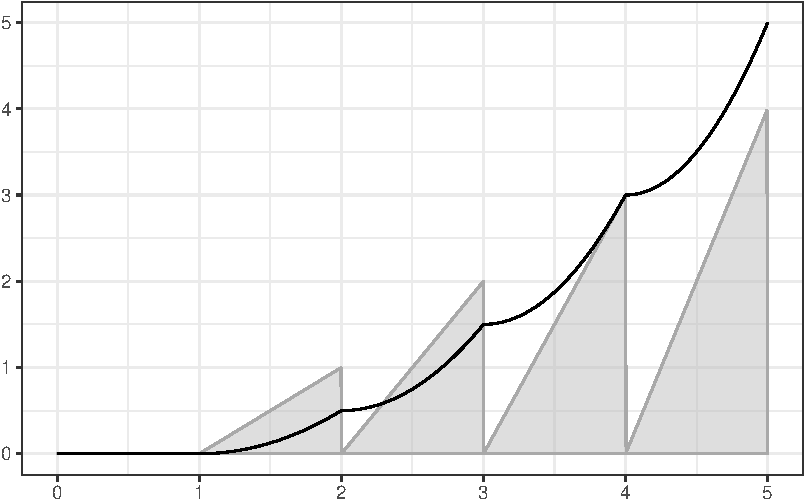
\includegraphics{book/03-Computación/index_files/figure-pdf/unnamed-chunk-3-1.pdf}

}

\caption{Producto de la función suelo y la parte entera}

\end{figure}

\begin{equation}\protect\hypertarget{eq-integralfunc1}{}{
\begin{multline}
I_{8}(x) = \int_0^x \left\lfloor t \right\rfloor \left\{ t \right\} dt
\end{multline}
}\label{eq-integralfunc1}\end{equation}

\begin{equation}\protect\hypertarget{eq-intsuelo1}{}{
\begin{multline}
t^2=(\left\lfloor t \right\rfloor + \left\{ t \right\})^2 =
{\left\lfloor t \right\rfloor}^{2} + 2 \left\lfloor t \right\rfloor \left\{ t \right\} + \left\{ t \right\}^2
\end{multline}
}\label{eq-intsuelo1}\end{equation}

\begin{equation}\protect\hypertarget{eq-intsuelo2}{}{
\begin{multline}
\left\lfloor t \right\rfloor \left\{ t \right\} = 
\frac{1}{2}(t^2 - \left\{ t \right\}^2 - \left\lfloor t \right\rfloor^{2})
\end{multline}
}\label{eq-intsuelo2}\end{equation}

Sustituyendo los resultados anteriores: Ecuación~\ref{eq-intsuelo2},
Ecuación~\ref{eq-integralfrac6} y \textbf{?@eq-integralsuelo2d} en
Ecuación~\ref{eq-integralfunc1}.

\begin{equation}\protect\hypertarget{eq-intsuelo3}{}{
\begin{multline}
I_{8}(x)=\frac{1}{2} ( \frac{x^3}{3} - I_{4}(x) - I_{6}(x))
\end{multline}
}\label{eq-intsuelo3}\end{equation}

\begin{equation}\protect\hypertarget{eq-intsuelo4}{}{
\begin{multline}
I_{8}(x) = \frac{1}{2} (\left\lfloor x \right\rfloor \left\{ x \right\}^{2} +
\frac{{\left\lfloor x \right\rfloor}^{2} - \left\lfloor x \right\rfloor}{2})
\end{multline}
}\label{eq-intsuelo4}\end{equation}

\begin{equation}\protect\hypertarget{eq-intsuelo5}{}{
\begin{multline}
I_{8}(x) = \int_{0}^{x}{\left\lfloor t \right\rfloor \left\{ t \right\} dt} =
\frac{1}{2} ( \left\lfloor x \right\rfloor \left\{ x \right\}^2 + \frac{{\left\lfloor x \right\rfloor}^{2} - \left\lfloor x \right\rfloor}{2})
\end{multline}
}\label{eq-intsuelo5}\end{equation}

\hypertarget{integral-definida-del-producto-de-las-funciones-suelo-y-techo}{%
\subsubsection{Integral definida del producto de las funciones suelo y
techo}\label{integral-definida-del-producto-de-las-funciones-suelo-y-techo}}

\begin{figure}

{\centering 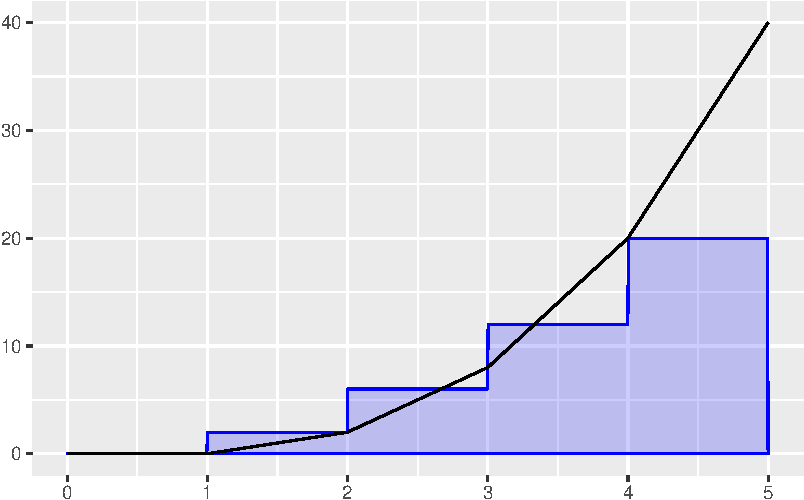
\includegraphics{book/03-Computación/index_files/figure-pdf/unnamed-chunk-4-1.pdf}

}

\caption{Producto de las funciones suelo y techo}

\end{figure}

\begin{equation}\protect\hypertarget{eq-integralfunc3}{}{
\begin{multline}
I_{9}(x) = \int_{0}^{x}{\left\lfloor t \right\rfloor \left\lceil  t \right\rceil dt}
\end{multline}
}\label{eq-integralfunc3}\end{equation}

La función\footnote{La función
  \(f(t) = \left\lfloor t \right\rfloor \left\lceil  t \right\rceil\),
  es simétrica respecto a origen \(f(-t)=f(t)\)}
\(f(t) = \left\lfloor t \right\rfloor \left\lceil  t \right\rceil\)
tiene una \emph{discontinuidad de primer orden} en cada \(f(n)\) si
\(n \in \mathbb{Z}\) y \(n \neq 0\), si calculamos los límites laterales
para un valor entero cualquiera, vemos que:

\begin{equation}\protect\hypertarget{eq-limits1}{}{
\begin{multline}
\left\{
\begin{array}{l}
  \quad \lim_{t \to n^{+}}{f(t)} = n(n+1) \\\\
  \quad \lim_{t \to n^{-}}{f(t)} = n(n-1) \\\\
  \quad f(n) = n^2 (n \in \mathbb{Z})
\end{array}
\right.
\end{multline}
}\label{eq-limits1}\end{equation}

Los límites laterales\footnote{Están relacionados con los \emph{números
  oblongos}, secuencia: \href{https://oeis.org/A002378}{A002378}} son
distintos en cada valor entero de la variable \(t\), salvo en el caso
\(t=0\).

\begin{equation}\protect\hypertarget{eq-limits2}{}{
\begin{multline}
\lim_{t \to n^{+}}{f(t)} \neq \lim_{t \to n^{-}}{f(t)}, n \in \mathbb{Z}-\{0\}
\end{multline}
}\label{eq-limits2}\end{equation}

\begin{equation}\protect\hypertarget{eq-integralfunc4ux29}{}{
\begin{multline}
I_{9}(x) = \int_{0}^{x}{\left\lfloor t \right\rfloor \left\lceil  t \right\rceil dt} =
\sum_{n=1}^{\left\lfloor x \right\rfloor-1}{n(n+1)} +
\int_{\left\lfloor x \right\rfloor}^{x}{\left\lfloor t \right\rfloor \left\lceil  t \right\rceil dt}
\end{multline}
}\label{eq-integralfunc4)}\end{equation}

\begin{equation}\protect\hypertarget{eq-integralfunc5}{}{
\begin{multline}
I_{9}(x) = 
\sum_{n=1}^{\left\lfloor x \right\rfloor-1}{n(n+1)} +
\left\lfloor x \right\rfloor \left\lceil  x \right\rceil (x-\left\lfloor x \right\rfloor) =
\end{multline}
}\label{eq-integralfunc5}\end{equation}

\begin{equation}\protect\hypertarget{eq-integralfunc6}{}{
\begin{multline}
I_{9}(x) = 
\frac{1}{3} (\left\lfloor x \right\rfloor-1)\left\lfloor x \right\rfloor(\left\lfloor x \right\rfloor-1) + 
\left\lfloor x \right\rfloor \left\lceil  x \right\rceil \left\{ x \right\}
\end{multline}
}\label{eq-integralfunc6}\end{equation}

\begin{equation}\protect\hypertarget{eq-integralfunc7}{}{
\begin{multline}
I_{9}(x) = \int_0^x \left\lfloor t \right\rfloor \left\lceil  t \right\rceil dt =
\left\lfloor x \right\rfloor \bigg(\frac{\left\lfloor x \right\rfloor^2-1}{3} + \left\lceil  x \right\rceil \left\{ x \right\}\bigg)
\end{multline}
}\label{eq-integralfunc7}\end{equation}

Otra forma alternativa de calcular la integral \(I_{9}(x)\) es sustituir
\(f(t) = \left\lfloor t \right\rfloor \left\lceil  t \right\rceil\) por
la función
\(g(t) = \left\lfloor t \right\rfloor^2 + \left\lfloor t \right\rfloor\)
que aunque difiere de \(f(x)\) para valores enteros, salvo \(t=0\), las
integrales coinciden ya que el conjunto de estas diferencias tienen una
medida nula.

Por lo que, utilizando los resultados Ecuación~\ref{eq-integralsuelo1} y
Ecuación~\ref{eq-integralsuelo2b}:

\begin{equation}\protect\hypertarget{eq-integralfunc8}{}{
\begin{multline}
I_{9}(x) = \int_0^x \left\lfloor t \right\rfloor \left\lceil  t \right\rceil dt =
\int_{0}^{x}{(\left\lfloor t \right\rfloor^{2} + \left\lfloor t \right\rfloor) dt} =
I_{6}(x) + I_{1}(x)
\end{multline}
}\label{eq-integralfunc8}\end{equation}

\begin{equation}\protect\hypertarget{eq-integralfunc9}{}{
\begin{multline}
I_{9}(x) = \int_0^x \left\lfloor t \right\rfloor \left\lceil  t \right\rceil dt =
\frac{1}{3} \left\lfloor x \right\rfloor (1 + \left\lfloor x \right\rfloor) (-1 + \left\lfloor x \right\rfloor + 3\left\{ x \right\})
\end{multline}
}\label{eq-integralfunc9}\end{equation}

\begin{itemize}
\tightlist
\item
  Código para \emph{Wolfram Mathematica}\footnote{Si simplificamos
    \(I_{6}(x) + I_{1}(x) - I_{9}(x)\) obtenemos
    \(\left\lfloor x \right\rfloor\left\{ x \right\}(1 - \left\lceil  x \right\rceil + \left\lfloor x \right\rfloor)\)
    que podemos comprobar que es \(0\) para cualquier valor de \(x\)}:
\end{itemize}

\begin{verbatim}
P[n_] := n*(n + 1)*(2 n + 1)/6
T[n_] := n*(n + 1)/2
I6[x_] := P[Floor[x] - 1] + FractionalPart[x]*(Floor[x]^2)
I1[x_] := Floor[x] * FractionalPart[x] + T[Floor[x] - 1]
Simplify[I6[x] + I1[x]]
\end{verbatim}

\hypertarget{integral-definida-de-la-funciuxf3n-suelo-del-cuadrado}{%
\subsubsection{Integral definida de la función suelo del
cuadrado}\label{integral-definida-de-la-funciuxf3n-suelo-del-cuadrado}}

\begin{equation}\protect\hypertarget{eq-integral2suelo1ux29}{}{
\begin{multline}
I_{10}(x) = \int_0^x \left\lfloor t^2 \right\rfloor dt
\end{multline}
}\label{eq-integral2suelo1)}\end{equation}

Observaciones:

\begin{itemize}
\item
  La función \(f(t)=\left\lfloor t^2 \right\rfloor\) tiene una
  \emph{discontinuidad de primer orden} en cada \(f(\sqrt{n})\) para
  todo \(n \in \mathbb{Z}\) y \(n \neq 0\)
\item
  \(f(t)\) es constante en el intervalo \([\sqrt(n), \sqrt(n+1)]\) para
  cualquier \(n\) entero, por lo que la integral definida en este
  intervalo equivale al área del rectángulo de base
  \(\sqrt{n+1} - \sqrt{n}\) y altura \(n\)
\end{itemize}

\begin{equation}\protect\hypertarget{eq-integral2suelo2}{}{
\begin{multline}
\int_{\sqrt{n}}^{\sqrt{n+1}} \left\lfloor t^2 \right\rfloor dt =
n (\sqrt{n+1} - \sqrt{n})
\end{multline}
}\label{eq-integral2suelo2}\end{equation}

\begin{equation}\protect\hypertarget{eq-integral2suelo3}{}{
\begin{multline}
\int_{\sqrt{n}}^{\sqrt{n+1}} \left\lfloor t^2 \right\rfloor dt =
n (\sqrt{n+1} - \sqrt{n})
\end{multline}
}\label{eq-integral2suelo3}\end{equation}

\begin{equation}\protect\hypertarget{eq-integral2suelo4}{}{
\begin{multline}
I_{10}(x) = \sum_{n=0}^{\sqrt{\left\lfloor x^2 \right\rfloor}}{\int_{\sqrt{n}}^{\sqrt{n+1}}{ \left\lfloor t^2 \right\rfloor dt}}  
+  \int_{\sqrt{\left\lfloor x^2 \right\rfloor}}^{x}{\left\lfloor t^2 \right\rfloor dt} = 
n (\sqrt{n+1} - \sqrt{n}) + x (x - \sqrt{\left\lfloor x^2 \right\rfloor})
\end{multline}
}\label{eq-integral2suelo4}\end{equation}

\hypertarget{ejercicios-de-integraciuxf3n-de-funciones-de-redondeo}{%
\subsection{Ejercicios de Integración de funciones de
redondeo}\label{ejercicios-de-integraciuxf3n-de-funciones-de-redondeo}}

\hypertarget{sumas-y-series.}{%
\subsection{Sumas y series.}\label{sumas-y-series.}}

\hypertarget{funciones-n-se-repite-fn-veces}{%
\section{\texorpdfstring{Funciones \(n\) se repite \(f(n)\)
veces}{Funciones n se repite f(n) veces}}\label{funciones-n-se-repite-fn-veces}}

\hypertarget{funciones-indexadoras.}{%
\section{Funciones indexadoras.}\label{funciones-indexadoras.}}

\hypertarget{funciuxf3n-muxf3dulo.}{%
\section{Función módulo.}\label{funciuxf3n-muxf3dulo.}}

\bookmarksetup{startatroot}

\hypertarget{funciones-aritmuxe9ticas}{%
\chapter{FUNCIONES ARITMÉTICAS}\label{funciones-aritmuxe9ticas}}

Revisando la bibliografía sobre \emph{Teoría de Números}, es difícil
encontrar una definición sobre lo que es una \emph{función aritmética}
que no sea vaga y difusa. Algunos autores las denominan, también,
funciones de la Teoría de Números.

Por ejemplo para (\textbf{apostol1998introduction?}), una función
aritmética es:

\emph{Una función real o compleja definida sobre los enteros positivos.}

En (\textbf{hardy2008introduction?}) se considera que:

\emph{Son funciones \(f(n)\) de un entero positivo definidas de cierta
forma que expresen ciertas propiedades aritméticas de \(n\)}

En (\textbf{cilleruelo1992?}), las funciones aritméticas son:

\emph{Ciertas funciones definidas sobre los naturales\ldots{} reales o
complejas}

En otros casos como el de (\textbf{vinogradov1977introduction?}), no se
da una definición y, simplemente, se las denomina:

\emph{``las funciones más importantes de la Teoría de Números''}

\hypertarget{definiciuxf3n}{%
\subsection{Definición}\label{definiciuxf3n}}

\hypertarget{tipos-de-funciones-aritmuxe9ticas}{%
\subsection{Tipos de funciones
aritméticas}\label{tipos-de-funciones-aritmuxe9ticas}}

\hypertarget{propiedades-1}{%
\subsection{Propiedades}\label{propiedades-1}}

\hypertarget{funciones-cluxe1sicas}{%
\subsection{Funciones clásicas}\label{funciones-cluxe1sicas}}

\hypertarget{convoluciuxf3n-recursiva-de-dirichlet}{%
\section{Convolución recursiva de
Dirichlet}\label{convoluciuxf3n-recursiva-de-dirichlet}}

\hypertarget{funciones-de-piltz}{%
\subsection{Funciones de Piltz}\label{funciones-de-piltz}}

\begin{multline}
\tau_{k}(n)=\sum_{d|n}{\tau_{k-1}(d)}
(\#eq:piltz1)
\end{multline}

\begin{multline}
\tau_{k}(n)=\prod_{i=1}^{\omega(n)}{\prod_{j=1}^{k-1}\frac{\alpha_{i}+j}{j}}=
\prod_{i=1}^{\omega(n)}{\binom{\alpha_{i}+k-1}{k-1}}; \; (k \ge 1)
(\#eq:piltz2)
\end{multline}

Si \(s\) es un número libre de factor cuadrado, véase secuencia
\href{https://oeis.org/A005117}{A005117}:

\begin{multline}
\tau_{k}(s)= \prod_{i=1}^{\omega(s)}{\binom{k}{k-1}=k^{\omega(s)}}
(\#eq:piltz3)
\end{multline}

\begin{multline}
\tau_{k+1}(n^k)=\tau_{k}(n^k)\cdot \tau_2(n); \; (k \ge 0)
(\#eq:piltz4)
\end{multline}

Secuencia \href{https://oeis.org/A097988}{A097988}

\begin{multline}
\tau_{3}(n)^{2}=\left( \sum_{d|n}{\tau_{2}(d)} \right)^{2}
(\#eq:piltz5)
\end{multline}

La función \(rad(n)\) se denomina el radical de \(n\) y es el producto
de los números primos que dividen a \(n\).
\href{https://oeis.org/A007947}{A007947}:

\begin{multline}
\tau_{k}(n)=\prod_{i=0}^{k-2}{\frac{ \tau_{2}(n\cdot rad(n)^{i}) }{ \tau_{2}(rad(n)^{i})}} ; \; (k \ge 1)
(\#eq:piltz6)
\end{multline}

Secuencia \href{https://oeis.org/A076479}{A076479}

\begin{multline}
\sum_{d|n}{\mu(d)\cdot\tau_{2}(d)}=
(-1)^{\omega(n)}=\mu(rad(n))
(\#eq:piltz7)
\end{multline}

\begin{multline}
\sum_{d|n}{{\mu(d)}^{2}\cdot{\tau_{2}(d)}^{k}}=
\tau_k(rad(n))=\bigg({2^{k}+1}\bigg)^{\omega(n)}
(\#eq:piltz8)
\end{multline}

Secuencia \href{https://oeis.org/A082476}{A082476} \begin{multline}
|\sum_{d|n}{\mu(d)\cdot\tau_{3}(d^{2})}|= \sum_{d|n}{{\mu(d)}^{2}\cdot{\tau_{2}(d)}^{2}}=
\tau_{5}(rad(n))=5^{\omega(n)}
(\#eq:piltz9)
\end{multline}

Secuencia \href{https://oeis.org/A010553}{A010553} \begin{multline}
\tau_{2}(\tau_{2}(rad(n)))-1=\omega(n) \; ; \; (n > 1)
(\#eq:piltz10)
\end{multline}

Secuencia \href{https://oeis.org/A074816}{A074816} \begin{multline}
\sum_{d|n}{ \mu(d)^{2} \cdot \tau_{2}(d) } =
|\sum_{d|n}{ \mu(d) \cdot \tau_{2}(d^3) }| =
|\sum_{d|n}{ \mu(d) \cdot \tau_{4}(d) }| =
\tau_{3}(rad(n)) =
3^{\omega(n)}
(\#eq:piltz11)
\end{multline}

\begin{multline}
|\sum_{d|n}{\mu(d)\cdot\tau_{k}(d^{m})}|=
{\bigg(\binom{k+m-1}{m}-1 \bigg)}^{\omega(n)}
(\#eq:piltz12)
\end{multline}

\begin{multline}
\sum_{d|n}{\mu(d)\cdot\tau_{k}(d^{m})}=
{\bigg(1-\binom{k+m-1}{m}\bigg) }^{\omega(n)}
(\#eq:piltz13)
\end{multline}

Secuencia \href{https://oeis.org/A000010}{A000010} \begin{multline}
\phi(n)=\sum_{i=1}^{n}{\bigg\lfloor \frac{\tau_{k}(i\cdot n)}{\tau_{k}(i)\cdot \tau_{k}(n)} \bigg\rfloor}
(\#eq:piltz14)
\end{multline}

Secuencia \href{https://oeis.org/A000720}{A000720} \begin{multline}
\pi(n)=
\sum_{i=2}^{n}{\bigg\lfloor \frac{k}{\tau_{k}(i)}\bigg\rfloor}
\;\; ;(n>1)
(\#eq:piltz15)
\end{multline}

Función de los divisores unitarios secuencia
\href{https://oeis.org/A034444}{A034444} \begin{multline}
\sigma_{0}^{*}(n)=
|\sum_{d|n}{\mu(d)\cdot\tau_{3}(d)}|=
\sum_{d|n}{{\mu(d)}^2}=
\sum_{d|n}{\mu\bigg(\frac{n}{d}\bigg)\cdot\tau_{2}(d^{2})}=
\sum_{d|n}{{\mu(d)}^2\cdot\tau_{2}(d^{2})}
(\#eq:piltz16)
\end{multline}

\begin{multline}
\tau_{k}(p^{\alpha})=
\binom{\alpha+k-1}{k-1}=
P_{k-1}^{ (\alpha,\beta) }(1) \; (k>1)
(\#eq:piltz17)
\end{multline}

Dónde, \(P_{n}^{ (\alpha,\beta) }(z)\) son los Polinomios de Jacobi

\begin{multline}
\sum_{d|n}{k^{\omega(n)}}=
\tau_{2}(n^{k})
(\#eq:piltz18)
\end{multline}

\hypertarget{funciones-de-jordan}{%
\subsection{Funciones de Jordan}\label{funciones-de-jordan}}

\hypertarget{funciuxf3n-lambda-de-liouville}{%
\subsection{Función Lambda de
Liouville}\label{funciuxf3n-lambda-de-liouville}}

\hypertarget{divisibilidad-entre-funciones-aritmuxe9ticas}{%
\section{Divisibilidad entre funciones
aritméticas}\label{divisibilidad-entre-funciones-aritmuxe9ticas}}

La divisibilidad entre distintas \emph{funciones aritméticas} crea unos
conjuntos de números con propiedades especiales que originan una serie
de problemas dignos de atención y que proporcionan una nueva perspectiva
de las propiedades de dichas funciones, y de su imagen.

\leavevmode\vadjust pre{\hypertarget{conjdiv}{}}%
Se denomina \emph{conjunto de divisibilidad} \(\mathcal{D}(f,g)\) entre
las funciones aritméticas \(f\) y \(g\) al formado por los números
\(n \in \mathbb{N}\) que cumplen que:

\begin{multline} 
n \in \mathcal{D}(f,g) \iff g(n) | f(n)
(\#eq:conjuntodiv1)
\end{multline}

\leavevmode\vadjust pre{\hypertarget{multconjdiv}{}}%
Si \(f\) y \(g\) son dos \emph{funciones aritméticas multiplicativas} y
si \(g(m)|f(n)\) y \(g(m)|f(n)\), con \(m \perp n\) entonces
\(g(n \cdot m) | f(n \cdot m)\) , y usando la notación de los conjuntos
de divisibilidad:
\(n, m \in \mathcal{D}(f,g) \land n \perp m \Rightarrow n \cdot m \in \mathcal{D}(f,g)\)

\leavevmode\vadjust pre{\hypertarget{unoconjdiv}{}}%
Si \(f\) y \(g\) son dos \emph{funciones aritméticas multiplicativas}:
\begin{multline} 
1 \in \mathcal{D}(f,g)
(\#eq:unoconjdiv)
\end{multline}

\leavevmode\vadjust pre{\hypertarget{conjindiv}{}}%
Se denomina \emph{conjunto de indivisibilidad} \(\mathcal{N}(f,g)\)
entre las funciones aritméticas \(f\) y \(g\) al formado por los números
\(n \in \mathbb{N}\) que cumplen que:

\begin{multline} 
n \in \mathcal{N}(f,g) \iff g(n) \nmid f(n)
(\#eq:conjuntoindiv1)
\end{multline}

\leavevmode\vadjust pre{\hypertarget{divnodiv}{}}%
Dadas dos funciones aritméticas \(f\) y \(g\), los conjuntos
\(\mathcal{D}(f,g)\) y \(\mathcal{N}(f,g)\)

\begin{multline}
\mathcal{D}(f,g) \cup \mathcal{N}(f,g) = \mathbb{N}
\mathcal{D}(f,g) \cap \mathcal{N}(f,g) = \emptyset
(\#eq:divnodiv)
\end{multline}

\hypertarget{acotaciuxf3n-de-funciones-aritmuxe9ticas}{%
\section{Acotación de funciones
aritméticas}\label{acotaciuxf3n-de-funciones-aritmuxe9ticas}}

\hypertarget{sumas-finitas-de-funciones-aritmuxe9ticas}{%
\section{Sumas finitas de funciones
aritméticas}\label{sumas-finitas-de-funciones-aritmuxe9ticas}}

\bookmarksetup{startatroot}

\hypertarget{ecuaciones-entre-funciones-aritmuxe9ticas}{%
\chapter{ECUACIONES ENTRE FUNCIONES
ARITMÉTICAS}\label{ecuaciones-entre-funciones-aritmuxe9ticas}}

Este tipo de problemas de \emph{Teoría de Números} proporciona una nueva
perspectiva del conjunto imagen de las funciones aritméticas. Para
buscar, las propiedades que presenta el conjunto solución, se debe
emplear todo tipo de herramientas matemáticas: desde elementales,
numéricas y analíticas. La mayoría de estos problemas han sido
estudiados ampliamente durante décadas, y existen numerosas referencias
bibliográficas a los mismos. Aunque, por otro lado, no es nada difícil
enunciar problemas originales de los que no existe documentación alguna.

El análisis de las ecuaciones que involucran funciones aritméticas
conlleva la exploración de las propiedades de las secuencias de números
enteros que conforman el conjunto de soluciones a estas ecuaciones.

\hypertarget{conjunto-soluciuxf3n-de-una-ecuaciuxf3n-entre-funciones-aritmuxe9ticas}{%
\section{Conjunto solución de una ecuación entre funciones
aritméticas}\label{conjunto-soluciuxf3n-de-una-ecuaciuxf3n-entre-funciones-aritmuxe9ticas}}

\hypertarget{conjsoleq}{}

\begin{equation}\protect\hypertarget{eq-prueba}{}{
\begin{multline} 
\mathcal{S} = \{n \in \mathbb{N^*} \mid g(n)=f(n)\}
\end{multline}
}\label{eq-prueba}\end{equation}

Referencia a una equación de prueba Ecuación~\ref{eq-prueba}

\hypertarget{ecuaciuxf3n-varphin-varphin-k}{%
\section{\texorpdfstring{Ecuación
\(\varphi(n) = \varphi(n + k)\)}{Ecuación \textbackslash varphi(n) = \textbackslash varphi(n + k)}}\label{ecuaciuxf3n-varphin-varphin-k}}

\begin{equation}\protect\hypertarget{eq-conjphiphi1}{}{
\begin{multline} 
\mathcal{S}_{k} = \{n \in \mathbb{N^*} \mid \varphi(n)=\varphi(n+k)\}
\end{multline}
}\label{eq-conjphiphi1}\end{equation}

\begin{longtable}[]{@{}
  >{\centering\arraybackslash}p{(\columnwidth - 6\tabcolsep) * \real{0.0412}}
  >{\centering\arraybackslash}p{(\columnwidth - 6\tabcolsep) * \real{0.1134}}
  >{\centering\arraybackslash}p{(\columnwidth - 6\tabcolsep) * \real{0.3093}}
  >{\raggedright\arraybackslash}p{(\columnwidth - 6\tabcolsep) * \real{0.5361}}@{}}
\toprule\noalign{}
\begin{minipage}[b]{\linewidth}\centering
k
\end{minipage} & \begin{minipage}[b]{\linewidth}\centering
Secuencia
\end{minipage} & \begin{minipage}[b]{\linewidth}\centering
Ecuación
\end{minipage} & \begin{minipage}[b]{\linewidth}\raggedright
Soluciones
\end{minipage} \\
\midrule\noalign{}
\endhead
\bottomrule\noalign{}
\endlastfoot
1 & \href{https://oeis.org/A001274/}{A001274} &
\(\varphi(n)=\varphi(n+1)\) &
\{1,3,15,104,164,194,255,495,584,975,\ldots\} \\
2 & \href{https://oeis.org/A001494/}{A001494} &
\(\varphi(n)=\varphi(n+2)\) & \{4,7,8,10,26,32,70,74,122,146,\ldots\} \\
3 & \href{https://oeis.org/A330251/}{A330251} &
\(\varphi(n)=\varphi(n+3)\) &
\{3,5,8720288051472,9134280520365,\ldots\} \\
4 & \href{https://oeis.org/A179186/}{A179186} &
\(\varphi(n)=\varphi(n+4)\) &
\{8,14,16,20,35,52,64,91,140,148,\ldots\} \\
5 & \href{https://oeis.org/A179187/}{A179187} &
\(\varphi(n)=\varphi(n+5)\) &
\{5,9,15,21,15556,21016,25930,25935,27027,36304,\ldots\} \\
6 & \href{https://oeis.org/A179188/}{A179188} &
\(\varphi(n)=\varphi(n+6)\) &
\{24,34,36,39,43,44,57,72,78,82,\ldots\} \\
7 & \href{https://oeis.org/A179189/}{A179189} &
\(\varphi(n)=\varphi(n+7)\) &
\{5,7,21,45,75,105,285,488,585,765,\ldots\} \\
8 & \href{https://oeis.org/A179202/}{A179202} &
\(\varphi(n)=\varphi(n+8)\) &
\{13,16,19,25,28,32,40,70,104,128,\ldots\} \\
9 & \href{https://oeis.org/A330429/}{A330429} &
\(\varphi(n)=\varphi(n+9)\) &
\{9,15,1005079920836,13695542245376,\ldots\} \\
10 & \href{https://oeis.org/A276503/}{A276503} &
\(\varphi(n)=\varphi(n+10)\) &
\{20,26,35,100,130,160,370,400,610,730,\ldots\} \\
11 & \href{https://oeis.org/A276504/}{A276504} &
\(\varphi(n)=\varphi(n+11)\) &
\{7,11,27,33,45,63,135,165,285,304,\ldots\} \\
12 & \href{https://oeis.org/A217139/}{A217139} &
\(\varphi(n)=\varphi(n+12)\) &
\{48,68,72,78,86,88,114,143,144,156,\ldots\} \\
\end{longtable}

\hypertarget{ecuaciuxf3n-varphin-k}{%
\section{\texorpdfstring{Ecuación
\(\varphi(n) = k\)}{Ecuación \textbackslash varphi(n) = k}}\label{ecuaciuxf3n-varphin-k}}

\hypertarget{ecuaciuxf3n-varphin-k-cdot-taun}{%
\section{\texorpdfstring{Ecuación
\(\varphi(n) = k \cdot \tau(n)\)}{Ecuación \textbackslash varphi(n) = k \textbackslash cdot \textbackslash tau(n)}}\label{ecuaciuxf3n-varphin-k-cdot-taun}}

\begin{longtable}[]{@{}
  >{\centering\arraybackslash}p{(\columnwidth - 6\tabcolsep) * \real{0.0370}}
  >{\centering\arraybackslash}p{(\columnwidth - 6\tabcolsep) * \real{0.1358}}
  >{\centering\arraybackslash}p{(\columnwidth - 6\tabcolsep) * \real{0.3951}}
  >{\raggedright\arraybackslash}p{(\columnwidth - 6\tabcolsep) * \real{0.4321}}@{}}
\toprule\noalign{}
\begin{minipage}[b]{\linewidth}\centering
k
\end{minipage} & \begin{minipage}[b]{\linewidth}\centering
Secuencia
\end{minipage} & \begin{minipage}[b]{\linewidth}\centering
Ecuación
\end{minipage} & \begin{minipage}[b]{\linewidth}\raggedright
Soluciones
\end{minipage} \\
\midrule\noalign{}
\endhead
\bottomrule\noalign{}
\endlastfoot
1 & \href{https://oeis.org/A020488/}{A020488} & \(\varphi(n)=\tau(n)\) &
\{1,3,8,10,18,24,30\} \\
2 & \href{https://oeis.org/A062516/}{A062516} &
\(\varphi(n) =2\cdot \tau(n)\) & \{5,9,15,28,40,72,84,90,120\} \\
3 & \href{https://oeis.org/A063469/}{A063469} &
\(\varphi(n) =3\cdot \tau(n)\) & \{7,21,26,56,70,78,108,126,168,210\} \\
4 & \href{https://oeis.org/A063470/}{A063470} &
\(\varphi(n) =4\cdot \tau(n)\) & \{34,45,52,102,140,156,252,360,420\} \\
\end{longtable}

\hypertarget{conjunto-soluciuxf3n}{%
\subsection{Conjunto solución}\label{conjunto-soluciuxf3n}}

\begin{equation}\protect\hypertarget{eq-conjphiktau}{}{
\begin{multline}
\mathcal{S}_{k} = \{n \in \mathbb{N^*} \mid \varphi(n)= k \cdot \tau(n)\}
\end{multline}
}\label{eq-conjphiktau}\end{equation}

\hypertarget{ecuaciuxf3n-varphin-taunk}{%
\section{\texorpdfstring{Ecuación
\(\varphi(n) = {\tau(n)}^{k}\)}{Ecuación \textbackslash varphi(n) = \{\textbackslash tau(n)\}\^{}\{k\}}}\label{ecuaciuxf3n-varphin-taunk}}

\hypertarget{tbl-cotbl-title:njphiktau1}{}
\begin{longtable}[]{@{}
  >{\centering\arraybackslash}p{(\columnwidth - 6\tabcolsep) * \real{0.0300}}
  >{\centering\arraybackslash}p{(\columnwidth - 6\tabcolsep) * \real{0.1100}}
  >{\centering\arraybackslash}p{(\columnwidth - 6\tabcolsep) * \real{0.3000}}
  >{\raggedright\arraybackslash}p{(\columnwidth - 6\tabcolsep) * \real{0.5600}}@{}}
\caption{\label{tbl-cotbl-title:njphiktau1}Ecuación
\(\varphi(n) = {\tau(n)}^{k}\)}\tabularnewline
\toprule\noalign{}
\begin{minipage}[b]{\linewidth}\centering
k
\end{minipage} & \begin{minipage}[b]{\linewidth}\centering
Secuencia
\end{minipage} & \begin{minipage}[b]{\linewidth}\centering
Ecuación
\end{minipage} & \begin{minipage}[b]{\linewidth}\raggedright
Soluciones
\end{minipage} \\
\midrule\noalign{}
\endfirsthead
\toprule\noalign{}
\begin{minipage}[b]{\linewidth}\centering
k
\end{minipage} & \begin{minipage}[b]{\linewidth}\centering
Secuencia
\end{minipage} & \begin{minipage}[b]{\linewidth}\centering
Ecuación
\end{minipage} & \begin{minipage}[b]{\linewidth}\raggedright
Soluciones
\end{minipage} \\
\midrule\noalign{}
\endhead
\bottomrule\noalign{}
\endlastfoot
1 & \href{https://oeis.org/A020488/}{A020488} &
\(\varphi(n)={\tau(n)}^{}\) & \{1,3,8,10,18,24,30\} \\
2 & \href{https://oeis.org/A068560/}{A068560} &
\(\varphi(n)={\tau(n)}^{2}\) &
\{1,5,34,63,76,128,136,170,315,364,\ldots\} \\
3 & \href{https://oeis.org/A068559/}{A068559} &
\(\varphi(n)={\tau(n)}^{3}\) &
\{1,85,333,436,1542,1875,2907,3285,3488,3796,\ldots\} \\
4 & \href{https://oeis.org/A114063/}{A114063} &
\(\varphi(n)={\tau(n)}^{4}\) &
\{1,17,514,8738,32301,33003,36351,41504,42292,43852,\ldots\} \\
\end{longtable}

\bookmarksetup{startatroot}

\hypertarget{summary}{%
\chapter{Summary}\label{summary}}

In summary, this book has no content whatsoever.

\begin{Shaded}
\begin{Highlighting}[]
\DecValTok{1} \SpecialCharTok{+} \DecValTok{1}
\end{Highlighting}
\end{Shaded}

\begin{verbatim}
[1] 2
\end{verbatim}

\bookmarksetup{startatroot}

\hypertarget{references}{%
\chapter*{References}\label{references}}
\addcontentsline{toc}{chapter}{References}

\markboth{References}{References}

\hypertarget{refs}{}
\begin{CSLReferences}{0}{0}
\end{CSLReferences}



\end{document}
